
%% bare_conf.tex
%% V1.3
%% 2007/01/11
%% by Michael Shell
%% See:
%% http://www.michaelshell.org/
%% for current contact information.
%%
%% This is a skeleton file demonstrating the use of IEEEtran.cls
%% (requires IEEEtran.cls version 1.7 or later) with an IEEE conference paper.
%% %% Support sites:
%% http://www.michaelshell.org/tex/ieeetran/
%% http://www.ctan.org/tex-archive/macros/latex/contrib/IEEEtran/
%% and
%% http://www.ieee.org/

%%*************************************************************************
%% Legal Notice:
%% This code is offered as-is without any warranty either expressed or
%% implied; without even the implied warranty of MERCHANTABILITY or
%% FITNESS FOR A PARTICULAR PURPOSE! 
%% User assumes all risk.
%% In no event shall IEEE or any contributor to this code be liable for
%% any damages or losses, including, but not limited to, incidental,
%% consequential, or any other damages, resulting from the use or misuse
%% of any information contained here.
%%
%% All comments are the opinions of their respective authors and are not
%% necessarily endorsed by the IEEE.
%%
%% This work is distributed under the LaTeX Project Public License (LPPL)
%% ( http://www.latex-project.org/ ) version 1.3, and may be freely used,
%% distributed and modified. A copy of the LPPL, version 1.3, is included
%% in the base LaTeX documentation of all distributions of LaTeX released
%% 2003/12/01 or later.
%% Retain all contribution notices and credits.
%% ** Modified files should be clearly indicated as such, including  **
%% ** renaming them and changing author support contact information. **
%%
%% File list of work: IEEEtran.cls, IEEEtran_HOWTO.pdf, bare_adv.tex,
%%                    bare_conf.tex, bare_jrnl.tex, bare_jrnl_compsoc.tex
%%*************************************************************************

% *** Authors should verify (and, if needed, correct) their LaTeX system  ***
% *** with the testflow diagnostic prior to trusting their LaTeX platform ***
% *** with production work. IEEE's font choices can trigger bugs that do  ***
% *** not appear when using other class files.                            ***
% The testflow support page is at:
% http://www.michaelshell.org/tex/testflow/



% Note that the a4paper option is mainly intended so that authors in
% countries using A4 can easily print to A4 and see how their papers will
% look in print - the typesetting of the document will not typically be
% affected with changes in paper size (but the bottom and side margins will).
% Use the testflow package mentioned above to verify correct handling of
% both paper sizes by the user's LaTeX system.
%
% Also note that the "draftcls" or "draftclsnofoot", not "draft", option
% should be used if it is desired that the figures are to be displayed in
% draft mode.
%
\documentclass[conference]{IEEEtran}
% Add the compsoc option for Computer Society conferences.
%
% If IEEEtran.cls has not been installed into the LaTeX system files,
% manually specify the path to it like:
% \documentclass[conference]{~/Dropbox/ResearchWu/AnalyticalProject/Conference/ConferenceStuff/Paper/IEEEtran2/IEEEtran}





% Some very useful LaTeX packages include:
% (uncomment the ones you want to load)


% *** MISC UTILITY PACKAGES ***
%
%\usepackage{ifpdf}
% Heiko Oberdiek's ifpdf.sty is very useful if you need conditional
% compilation based on whether the output is pdf or dvi.
% usage:
% \ifpdf
%   % pdf code
% \else
%   % dvi code
% \fi
% The latest version of ifpdf.sty can be obtained from:
% http://www.ctan.org/tex-archive/macros/latex/contrib/oberdiek/
% Also, note that IEEEtran.cls V1.7 and later provides a builtin
% \ifCLASSINFOpdf conditional that works the same way.
% When switching from latex to pdflatex and vice-versa, the compiler may
% have to be run twice to clear warning/error messages.






% *** CITATION PACKAGES ***
%
\usepackage{cite}
% cite.sty was written by Donald Arseneau
% V1.6 and later of IEEEtran pre-defines the format of the cite.sty package
% \cite{} output to follow that of IEEE. Loading the cite package will
% result in citation numbers being automatically sorted and properly
% "compressed/ranged". e.g., [1], [9], [2], [7], [5], [6] without using
% cite.sty will become [1], [2], [5]--[7], [9] using cite.sty. cite.sty's
% \cite will automatically add leading space, if needed. Use cite.sty's
% noadjust option (cite.sty V3.8 and later) if you want to turn this off.
% cite.sty is already installed on most LaTeX systems. Be sure and use
% version 4.0 (2003-05-27) and later if using hyperref.sty. cite.sty does
% not currently provide for hyperlinked citations.
% The latest version can be obtained at:
% http://www.ctan.org/tex-archive/macros/latex/contrib/cite/
% The documentation is contained in the cite.sty file itself.
\usepackage{multicol}





% *** GRAPHICS RELATED PACKAGES ***
%
%\ifCLASSINFOpdf
  % \usepackage[pdftex]{graphicx}
  % declare the path(s) where your graphic files are
  % \graphicspath{{../pdf/}{../jpeg/}}
  % and their extensions so you won't have to specify these with
  % every instance of \includegraphics
  % \DeclareGraphicsExtensions{.pdf,.jpeg,.png}
%\else
  % or other class option (dvipsone, dvipdf, if not using dvips). graphicx
  % will default to the driver specified in the system graphics.cfg if no
  % driver is specified.
  % \usepackage[dvips]{graphicx}
  % declare the path(s) where your graphic files are
  % \graphicspath{{../eps/}}
  % and their extensions so you won't have to specify these with
  % every instance of \includegraphics
  % \DeclareGraphicsExtensions{.eps}
%\fi
% graphicx was written by David Carlisle and Sebastian Rahtz. It is
% required if you want graphics, photos, etc. graphicx.sty is already
% installed on most LaTeX systems. The latest version and documentation can
% be obtained at: 
% http://www.ctan.org/tex-archive/macros/latex/required/graphics/
% Another good source of documentation is "Using Imported Graphics in
% LaTeX2e" by Keith Reckdahl which can be found as epslatex.ps or
% epslatex.pdf at: http://www.ctan.org/tex-archive/info/
%
% latex, and pdflatex in dvi mode, support graphics in encapsulated
% postscript (.eps) format. pdflatex in pdf mode supports graphics
% in .pdf, .jpeg, .png and .mps (metapost) formats. Users should ensure
% that all non-photo figures use a vector format (.eps, .pdf, .mps) and
% not a bitmapped formats (.jpeg, .png). IEEE frowns on bitmapped formats
% which can result in "jaggedy"/blurry rendering of lines and letters as
% well as large increases in file sizes.
%
% You can find documentation about the pdfTeX application at:
% http://www.tug.org/applications/pdftex





% *** MATH PACKAGES ***
%
\usepackage[cmex10]{amsmath}
% A popular package from the American Mathematical Society that provides
% many useful and powerful commands for dealing with mathematics. If using
% it, be sure to load this package with the cmex10 option to ensure that
% only type 1 fonts will utilized at all point sizes. Without this option,
% it is possible that some math symbols, particularly those within
% footnotes, will be rendered in bitmap form which will result in a
% document that can not be IEEE Xplore compliant!
%
% Also, note that the amsmath package sets \interdisplaylinepenalty to 10000
% thus preventing page breaks from occurring within multiline equations. Use:
\interdisplaylinepenalty=2500
% after loading amsmath to restore such page breaks as IEEEtran.cls normally
% does. amsmath.sty is already installed on most LaTeX systems. The latest
% version and documentation can be obtained at:
% http://www.ctan.org/tex-archive/macros/latex/required/amslatex/math/





% *** SPECIALIZED LIST PACKAGES ***
%
%\usepackage{algorithmic}
% algorithmic.sty was written by Peter Williams and Rogerio Brito.
% This package provides an algorithmic environment fo describing algorithms.
% You can use the algorithmic environment in-text or within a figure
% environment to provide for a floating algorithm. Do NOT use the algorithm
% floating environment provided by algorithm.sty (by the same authors) or
% algorithm2e.sty (by Christophe Fiorio) as IEEE does not use dedicated
% algorithm float types and packages that provide these will not provide
% correct IEEE style captions. The latest version and documentation of
% algorithmic.sty can be obtained at:
% http://www.ctan.org/tex-archive/macros/latex/contrib/algorithms/
% There is also a support site at:
% http://algorithms.berlios.de/index.html
% Also of interest may be the (relatively newer and more customizable)
% algorithmicx.sty package by Szasz Janos:
% http://www.ctan.org/tex-archive/macros/latex/contrib/algorithmicx/




% *** ALIGNMENT PACKAGES ***
%
% \usepackage{array}
% Frank Mittelbach's and David Carlisle's array.sty patches and improves
% the standard LaTeX2e array and tabular environments to provide better
% appearance and additional user controls. As the default LaTeX2e table
% generation code is lacking to the point of almost being broken with
% respect to the quality of the end results, all users are strongly
% advised to use an enhanced (at the very least that provided by array.sty)
% set of table tools. array.sty is already installed on most systems. The
% latest version and documentation can be obtained at:
% http://www.ctan.org/tex-archive/macros/latex/required/tools/


%\usepackage{mdwmath}
%\usepackage{mdwtab}
% Also highly recommended is Mark Wooding's extremely powerful MDW tools,
% especially mdwmath.sty and mdwtab.sty which are used to format equations
% and tables, respectively. The MDWtools set is already installed on most
% LaTeX systems. The lastest version and documentation is available at:
% http://www.ctan.org/tex-archive/macros/latex/contrib/mdwtools/


% IEEEtran contains the IEEEeqnarray family of commands that can be used to
% generate multiline equations as well as matrices, tables, etc., of high
% quality.


%\usepackage{eqparbox}
% Also of notable interest is Scott Pakin's eqparbox package for creating
% (automatically sized) equal width boxes - aka "natural width parboxes".
% Available at:
% http://www.ctan.org/tex-archive/macros/latex/contrib/eqparbox/





% *** SUBFIGURE PACKAGES ***
%\usepackage[tight,footnotesize]{subfigure}
% subfigure.sty was written by Steven Douglas Cochran. This package makes it
% easy to put subfigures in your figures. e.g., "Figure 1a and 1b". For IEEE
% work, it is a good idea to load it with the tight package option to reduce
% the amount of white space around the subfigures. subfigure.sty is already
% installed on most LaTeX systems. The latest version and documentation can
% be obtained at:
% http://www.ctan.org/tex-archive/obsolete/macros/latex/contrib/subfigure/
% subfigure.sty has been superceeded by subfig.sty.



%\usepackage[caption=false]{caption}
%\usepackage[font=footnotesize]{subfig}
% subfig.sty, also written by Steven Douglas Cochran, is the modern
% replacement for subfigure.sty. However, subfig.sty requires and
% automatically loads Axel Sommerfeldt's caption.sty which will override
% IEEEtran.cls handling of captions and this will result in nonIEEE style
% figure/table captions. To prevent this problem, be sure and preload
% caption.sty with its "caption=false" package option. This is will preserve
% IEEEtran.cls handing of captions. Version 1.3 (2005/06/28) and later 
% (recommended due to many improvements over 1.2) of subfig.sty supports
% the caption=false option directly:
%\usepackage[caption=false,font=footnotesize]{subfig}
%
% The latest version and documentation can be obtained at:
% http://www.ctan.org/tex-archive/macros/latex/contrib/subfig/
% The latest version and documentation of caption.sty can be obtained at:
% http://www.ctan.org/tex-archive/macros/latex/contrib/caption/


\usepackage{graphicx}
% *** FLOAT PACKAGES ***
%
%\usepackage{fixltx2e}
% fixltx2e, the successor to the earlier fix2col.sty, was written by
% Frank Mittelbach and David Carlisle. This package corrects a few problems
% in the LaTeX2e kernel, the most notable of which is that in current
% LaTeX2e releases, the ordering of single and double column floats is not
% guaranteed to be preserved. Thus, an unpatched LaTeX2e can allow a
% single column figure to be placed prior to an earlier double column
% figure. The latest version and documentation can be found at:
% http://www.ctan.org/tex-archive/macros/latex/base/



%\usepackage{stfloats}
% stfloats.sty was written by Sigitas Tolusis. This package gives LaTeX2e
% the ability to do double column floats at the bottom of the page as well
% as the top. (e.g., "\begin{figure*}[!b]" is not normally possible in
% LaTeX2e). It also provides a command:
%\fnbelowfloat
% to enable the placement of footnotes below bottom floats (the standard
% LaTeX2e kernel puts them above bottom floats). This is an invasive package
% which rewrites many portions of the LaTeX2e float routines. It may not work
% with other packages that modify the LaTeX2e float routines. The latest
% version and documentation can be obtained at:
% http://www.ctan.org/tex-archive/macros/latex/contrib/sttools/
% Documentation is contained in the stfloats.sty comments as well as in the
% presfull.pdf file. Do not use the stfloats baselinefloat ability as IEEE
% does not allow \baselineskip to stretch. Authors submitting work to the
% IEEE should note that IEEE rarely uses double column equations and
% that authors should try to avoid such use. Do not be tempted to use the
% cuted.sty or midfloat.sty packages (also by Sigitas Tolusis) as IEEE does
% not format its papers in such ways.





% *** PDF, URL AND HYPERLINK PACKAGES ***
%
%\usepackage{url}
% url.sty was written by Donald Arseneau. It provides better support for
% handling and breaking URLs. url.sty is already installed on most LaTeX
% systems. The latest version can be obtained at:
% http://www.ctan.org/tex-archive/macros/latex/contrib/misc/
% Read the url.sty source comments for usage information. Basically,
% \url{my_url_here}.





% *** Do not adjust lengths that control margins, column widths, etc. ***
% *** Do not use packages that alter fonts (such as pslatex).         ***
% There should be no need to do such things with IEEEtran.cls V1.6 and later.
% (Unless specifically asked to do so by the journal or conference you plan
% to submit to, of course. )


% correct bad hyphenation here
\hyphenation{op-tical net-works semi-conduc-tor}


\begin{document}
%
% paper title
% can use linebreaks \\ within to get better formatting as desired
\title{Chaos in the Electric Curtain}


% author names and affiliations
% use a multiple column layout for up to three different
% affiliations
\author{\IEEEauthorblockN{Owen Myers}
\IEEEauthorblockA{Materials Science Program\\
University of Vermont\\
Burlington, Vermont 05405\\
Email: Oweenm@gmail.com}

\and
\IEEEauthorblockN{Junru Wu, Ph.D.}
\IEEEauthorblockA{Department of Physics\\Materials Science Program\\
University of Vermont\\
Burlington, Vermont 05405\\
Email: Jun-Ru.Wu@uvm.edu\\
Web Page:\\
http://www.uvm.edu/~jwu/Wu.html}
\and
\IEEEauthorblockN{Jeffrey Marshall Ph.D.}
\IEEEauthorblockA{School of Engineering\\
University of Vermont\\
Burlington, Vermont 05405\\
Email: JMasha1.edu\\
Web Page:\\
http://www.cems.uvm.edu/~jeffm/Research}}

% conference papers do not typically use \thanks and this command
% is locked out in conference mode. If really needed, such as for
% the acknowledgment of grants, issue a \IEEEoverridecommandlockouts
% after \documentclass

% for over three affiliations, or if they all won't fit within the width
% of the page, use this alternative format:
% 
%\author{\IEEEauthorblockN{Michael Shell\IEEEauthorrefmark{1},
%Homer Simpson\IEEEauthorrefmark{2},
%James Kirk\IEEEauthorrefmark{3}, 
%Montgomery Scott\IEEEauthorrefmark{3} and
%Eldon Tyrell\IEEEauthorrefmark{4}}
%\IEEEauthorblockA{\IEEEauthorrefmark{1}School of Electrical and Computer Engineering\\
%Georgia Institute of Technology,
%Atlanta, Georgia 30332--0250\\ Email: see http://www.michaelshell.org/contact.html}
%\IEEEauthorblockA{\IEEEauthorrefmark{2}Twentieth Century Fox, Springfield, USA\\
%Email: homer@thesimpsons.com}
%\IEEEauthorblockA{\IEEEauthorrefmark{3}Starfleet Academy, San Francisco, California 96678-2391\\
%Telephone: (800) 555--1212, Fax: (888) 555--1212}
%\IEEEauthorblockA{\IEEEauthorrefmark{4}Tyrell Inc., 123 Replicant Street, Los Angeles, California 90210--4321}}


% make the title area
\maketitle
\begin{abstract}
The Electric Curtain (EC) consists of a series of parallel electrodes embedded in a dielectric
surface driven by a multiphase alternating electric (AC) voltage source. The EC can transport
particles of a variety of materials, and it shows significant promise for dust mitigation and
separation applications with charged particles. In this paper, we use a simple mathematical model to
demonstrate interesting chaotic behavior of the particles in a EC 
field. We have identified multiple mode bifurcations as well as the onset of chaotic dynamics of
particle motion based on analysis of phase-plane plots, bifurcation diagrams and Poincar$\acute{e}$
sections. These bifurcations lead to abrupt changes in particle transport properties, such as average
translation velocity and elevation height. It may be possible to utilize this information to better
understand and control particle transport and/or separation efficiency on the EC by manipulating key
physical parameters to trigger or avoid bifurcations. We have further investigated some particle
trajectories in phase space when they are on the surface of the EC and briefly describe some
interesting behavior of the out-of-plane particle motion.
\end{abstract}
% no \IEEEPARstart
% You must have at least 2 lines in the paragraph with the drop letter
% (should never be an issue)


%.ran.cls defaults to using nonbold math in the Abstract.
% This preserves the distinction between vectors and scalars. However,
% if the conference you are submitting to favors bold math in the abstract,
% then you can use LaTeX's standard command \boldmath at the very start
% of the abstract to achieve this. Many IEEE journals/conferences frown on
% math in the abstract anyway.

% no keywords




% For peer review papers, you can put extra information on the cover
% page as needed:
% \ifCLASSOPTIONpeerreview
% \begin{center} \bfseries EDICS Category: 3-BBND \end{center}
% \fi
%
% For peerreview papers, this IEEEtran command inserts a page break and
% creates the second title. It will be ignored for other modes.
\IEEEpeerreviewmaketitle



\section{Introduction}
The Electric Curtain (EC) was patented in 1974 by Senichi Masuda for particles  position
manipulation and containment in an electrostatic powder painting application \cite{patent}. A simple
depiction of the EC is shown in Fig. \ref{simpleEC}. The EC is a series of parallel electrodes that are often
embedded in a dielectric surface. A standing wave electric field can be created above
the surface by applying a multiphase AC power source to each of the electrodes, and adjusting the
phase of this power source between neighboring electrodes to produce the desired wave form.  This
technique's primary advantage is its simplicity, allowing variations in the electric field above the
surface by changing the phase difference between electrodes or the waveforms of the AC voltage applied to
them without having to alter the physical apparatus. Whereas most methods for particle
transport or separation break down when the particles become charged, the EC relies on particle
charge for its operation. The EC has been examined in the context of many different applications.
For example, it has been used for separation of cells in solution \cite{blood}, separation of different
types of by-products from agricultural processes \cite{weiss}, transport of toner particles in
photocopying machines \cite{fredpatent}, mitigation of charged dust build-up for extra-terrestrial exploration of
dusty planets and moons \cite{dustshield}, and separation of charged particles with different
charge-to-mass ratios using a variety of EC designs \cite{sepkawamoto08}.

The motion of particles on an electric curtain has been studied both experimentally and
computationally by a number of investigators.
\cite{kawamoto,jeff,dudziczlaser,fredmodes,frednolev,hemstreetveldist,3phaseveldist}
These investigations have indicated that particles
exhibit various different modes of motion on the electric curtain, and they have illustrated how
each of these modes produces net motion of the particles. While we use a similar computational
approach to some of these previous papers, the current paper has a substantially different objective. Namely,
rather than focusing on the net particle motion, we seek to examine the
motion from a dynamical systems point of view. With this approach we work to develop greater
insight into sudden changes in the nature of particle transport that is sometimes observed in EC
particle transport, such as the intermittent changes in particle motion observed in a discrete-element
simulation of particle transport on an inclined EC by Chesnutt and Marshall\cite{chesnutt}. The onset of
chaotic motion of the particle is particularly of interest to us, given the close relationship of
chaotic motion and efficient mixing in particulate and fluid systems \cite{ottino}.  

\setlength{\unitlength}{1mm} 
\begin{figure}[!b] 
    \centering 
    \begin{picture}(50,25) 
        \put(5,15){\circle*{5}} 
        \put(15,15){\circle*{5}} 
        \put(25,15){\circle*{5}} 
        \put(35,15){\circle*{5}} 
        \put(45,15){\circle*{5}} 
        \put(5,17.5){$Electrodes$} 
        \put(0,20){\line(1,0){50}} 
        \put(0,20){\line(0,-1){10}} 
        \put(0,10){\line(1,0){50}} 
        \put(50,10){\line(0,1){10}} 
        \put(7.5,21){$Dielectric$ $Surface$} 
        \put(5,15){\line(0,-1){10}} 
        \put(15,15){\line(0,-1){10}} 
        \put(25,15){\line(0,-1){10}} 
        \put(35,15){\line(0,-1){10}} 
        \put(45,15){\line(0,-1){7.5}} 
        \put(5,5){\line(1,0){32.5}} 
        \put(37.5,0){\line(0,1){7.5}} 
        \put(50,0){\line(0,1){7.5}} 
        \put(37.5,0){\line(1,0){12.5}} 
        \put(37.5,7.5){\line(1,0){12.5}} 
        \put(38,4.5){{\tiny Multi-phase}} 
        \put(38,2.5){{\tiny AC Power}} 
        \put(38,.5){{\tiny Source}} 
    \end{picture} 
    \caption{Side view of electric curtain}
    \label{simpleEC}
\end{figure} 


\section{methods}
Three mathematical models were used by Masuda and Kamimura \cite{masudaapx} for determining the electrostatic
field above the EC surface. The calculations presented in this paper use the
so-called center line charge approximation, in which each electrode is approximated as a thin wire.
The electrostatic field is assumed to have a standing wave (2-phase) form, such that the phase
difference between adjacent electrodes is $180^{\circ}$. The approximate $x-$ and $y-$components of the
electric field for a 2-phase EC are given by
%
\begin{equation}
    E_x=\frac{k Q}{4\pi\epsilon_0} \sum_{n=0}^{1} \frac{\sin(k x - n \pi) \cos(\omega t - n
        \pi)}{\cosh(k y) - \cos(k x - n\pi)}
    \label{2phaseEx}
\end{equation}
%
\begin{equation}
    E_y = \frac{k Q}{4 \pi \epsilon_0}\sum_{n=0}^{1} \frac{\sinh(k y) \cos(\omega t - n
        \pi)}{\cosh(k y) - \cos(k x - n\pi )}
    \label{2phaseEy}
\end{equation}
%
where $Q$ is the charge amplitude on an electrode, $q$ and $m$ are the particle charge and mass,
respectively, $k$ is the wave number, and $\omega$ is the driving frequency \cite{masudaapx}.  In the cross-sectional plane
orthogonal to the electrode axis, the $x-$ and $y-$axes of a Cartesian coordinate system are parallel
and perpendicular to the dielectric surface, respectively.

In this initial investigation of bifurcations and chaotic dynamics of the particles on an EC, we
have confined attention to a highly simplified mathematical model of the particle dynamics. Primarily
we have looked at single particle motion on the EC surface for the case where the particle rolls on
the dielectric surface of the EC. This one-dimensional (1D) model offers the advantage of simple phase
diagrams and system analysis. We have also performed a preliminary investigation of two-dimensional
(2D) particle dynamics on the EC, for which case the particle is allowed to rise off the
dielectric surface. In both cases, Poincar$\acute{e}$ sections are used to simplify the phase space and search
for underlying order. In the one-dimensional case, we have also looked for the onset of chaos
through a sequence of period doubling. 

Dissipative forces are included in both the one- and two-dimensional models. For the 1D case,
particles roll along the dielectric surface, so the dissipative forces arise from both rolling
resistance and viscous fluid force (Stokes drag). Both of these two forces are proportional to the particle
velocity \cite{ballsurf}, so they are combined into one term in the particle equations of motion.  In
the 2D case,
the particle is assumed to be levitated with non-dissipative collisions with the dielectric
surface, so the only dissipation comes from fluid drag. The full differential equations governing
the particle's trajectory are
\begin{equation}
%    \begin{split}
        \frac{d^2x}{dt^2}+\frac{\beta}{m}\frac{dx}{dt}=
            \sum_{n=0}^{1} J \frac{\sin(k x - n\pi ) \cos(\omega t - n\pi)}{\cosh(k y) - \cos(k x - n\pi)} \\
%    \end{split}
    \label{2ndorderdiffeqx}
\end{equation}
\begin{equation}
%    \begin{split}
        \frac{d^2y}{dt^2} +\frac{\beta}{m}\frac{dy}{dt}=
            \sum_{n=0}^{1} J \frac{\sinh(k y) \cos(\omega t-n\pi)}{\cosh(k y)-\cos(k x-n\pi )}-g \\
%    \end{split}
    \label{2ndorderdiffeqy}
\end{equation}
where $J=kqQ/4 m \pi \epsilon_0$ is called the interaction amplitude, $\beta$ is the damping
coefficient, $m$ is the particle's mass, and $g$ is the acceleration due to gravity. In the
computations presented, the
variables are non-dimensionalized to simplify the numerical analysis. The non-dimensionalized
variables and parameters are expressed in terms of their dimensional counterparts as
\begin{multicols}{2}
\begin{itemize}
\item[] $t'=\omega t$
\item[] $x'=k x$
\item[] $y'=k y$
\item[] $j=\frac{k^2 q Q}{4\pi \epsilon_0 m^2 \omega^2}$
\item[] $g'=\frac{g k}{\omega^2}$
\item[] $\beta'=\frac{\beta}{m \omega}$
\end{itemize}
\end{multicols}
\noindent
The distance between neighboring electrodes is equal to
$\pi$ and the period of oscillation is equal to $2\pi$. The equations of motion can then be written
in dimensionless form as 
\begin{equation}
%    \begin{split}
        \frac{d^2x'}{dt'^2}+\beta'\frac{dx'}{dt'}= \sum_{n=0}^{1} j \frac{\sin(x' - n\pi ) \cos(t' - n\pi)}{\cosh(y') - \cos(x' - n\pi)} 
%    \end{split}
    \label{nondimeqx}
\end{equation}
\begin{equation}
%    \begin{split}
        \frac{d^2y'}{dt'^2} +\beta'\frac{dy'}{dt'}=
            \sum_{n=0}^{1} j \frac{\sinh(y') \cos(t' - n\pi)}{\cosh(y')-\cos(x' - n\pi )}-g' 
%    \end{split}
    \label{nondimeqy}
\end{equation}
For the 1D case, the value of $y'$ in equations (\ref{nondimeqx}) and (\ref{nondimeqy}) is set equal
to the centroid position of the rolling particles. The electric field approximation equations
(\ref{2phaseEx}) and (\ref{2phaseEy}) use singular (point) electrodes, and therefore only accurately
represent a physical system of cylindrical electrodes at a sufficiently far distance from the
electrodes. To insure that the electrodes are considered far from the particles, the dielectric
surface is specified to lie at a distance $y'=1$ above the plane of the array of electrodes.
Various tests have found this to be adequately far so that the
point-electrode approximation is well satisfied. Also, in the 1D study we need to consider values of
the parameter $j$ for which the particles remain on the surface, whereas for the 2D tests we wish to
select $j$ such that particles are levitated from the surface, with occasional collisions.  The
critical value of $j$ at which particles transition from 1D motion along the surface to 2D motion off of
the surface is determined by putting a particle directly above an electrode with a
repulsive interaction and solving for when the electrostatic force balances the gravitational
force. We can use the non-dimesionalized equations if we solve for the dimensionless ratio $j/g'$.
This will give us a critical relationship that will define the range of $j$ that the 1D
model is valid. The acceleration balance equation to be solved at the surface directly above an
electrode is
\begin{equation}
    \sum_{n=0}^{1} j \frac{\sinh(y') \cos(t' - n\pi)}{\cosh(y')-\cos(x' - n\pi )}=g' \\
\end{equation}
For a particle located over the electrode at $x'=0$ the expression simplifies to
\begin{equation}
   j\frac{2 \cos(t')\cosh(y')}{\cosh^2(y')-1}=g' 
\end{equation}
Therefore the inequality
\begin{equation}
    \frac{j}{g'}\leq \frac{\cosh^2(y')-1}{2 \cos(t')\cosh(y')}
\end{equation}
needs to be satisfied for the particle to remain on the surface.
The right hand side of the inequality is minimized when $\cos(t')=1$. Setting $\cos(t')$ to its
maximum value and setting the location of the surface as $y'=1$ we
find that $j/g'\approx0.448$ is the critical ratio that needs
to be considered. For these parameters the 1D model is valid if $j/g'<0.448$. In light of
this critical relationship we have
chosen $g'$ such that this criterion is satisfied for $0<j<2$.
It follows that the 2D model is appropriate for $.j/g'>0.448$ and in this paper we report on
interesting findings for $j/g'\approx3.06$.

\section{The One Dimensional Electric Curtain}

The 2-phase EC has two fixed points in the electric field, one located above each electrode. A
particle placed directly above an electrode in the 1D system therefore does not move even as the field
oscillates in time. The stability of the particle at these locations oscillates with the field. When
the charge of the electrode has the same sign of as the particle, the fixed point is unstable
because of the repulsion, whereas a particle above an electrode of the same sign charge lies in a
stable fixed point.  Interestingly, chaotic motion is known to occur in systems that have one stable
and one unstable fixed point, which suggests that the 1D EC may present interesting dynamics arising
from stability oscillation of these fixed points.

For purposes of analysis, it is convenient to express the governing equation
(\ref{2ndorderdiffeqx}) for the 1D model as a
set of first-order autonomous differential equations. This can be done by defining three variables,
$x_1$, $x_2$, and $x_3$, by $x_1=x'$, $x_2=\frac{dx'}{dt'}$, and $x_3=t'$. Equation
(\ref{2ndorderdiffeqx}) can then be expressed by
%
\begin{equation}
    \begin{split}
    &\dot{x}_1 = x_2 \\
    &\dot{x}_2 = \sum_{n=0}^{1} j \frac{\sin(x_1 - n\pi) \cos(x_3 - n
            \pi)}{\cosh(y') - \cos(x_1 - n\pi)} - \beta'x_2\\
    &\dot{x}_3 = 1 \\
    \end{split}
\end{equation}
%
When cast in this form, the periodic conditions in time and space ($x'$) can be employed to represent
the system dynamics within a bounded region in phase space. In all test cases reported for the 1D EC
the damping coefficient $\beta'$ is set equal to $0.1$ for simplicity.

\subsection{Poincar$\acute{e}$ Sections}

The trajectory (or orbit) of a particle in the three-dimensional phase space is obtained by plotting
the three coordinates $x_1$, $x_2$, and $x_3$, as shown in Fig. 2. The orbit of the particle in phase space
is usually quite dense, and it is not easy to discern much useful information about the system
dynamics directly from such a plot. Valuable insight into the system dynamics can be gained by a
Poincar$\acute{e}$ section, which is simply a cross-section of the particle orbit in phase space where we only
plot the points for which the particle trajectory is traveling in a specified direction through the
plane. Depending on the particular plane and direction selected the shape of the Poincar$\acute{e}$ section
may differ, but certain structural characteristics of the system will tend to remain the same. 

\begin{figure}[!t]
    \centering
    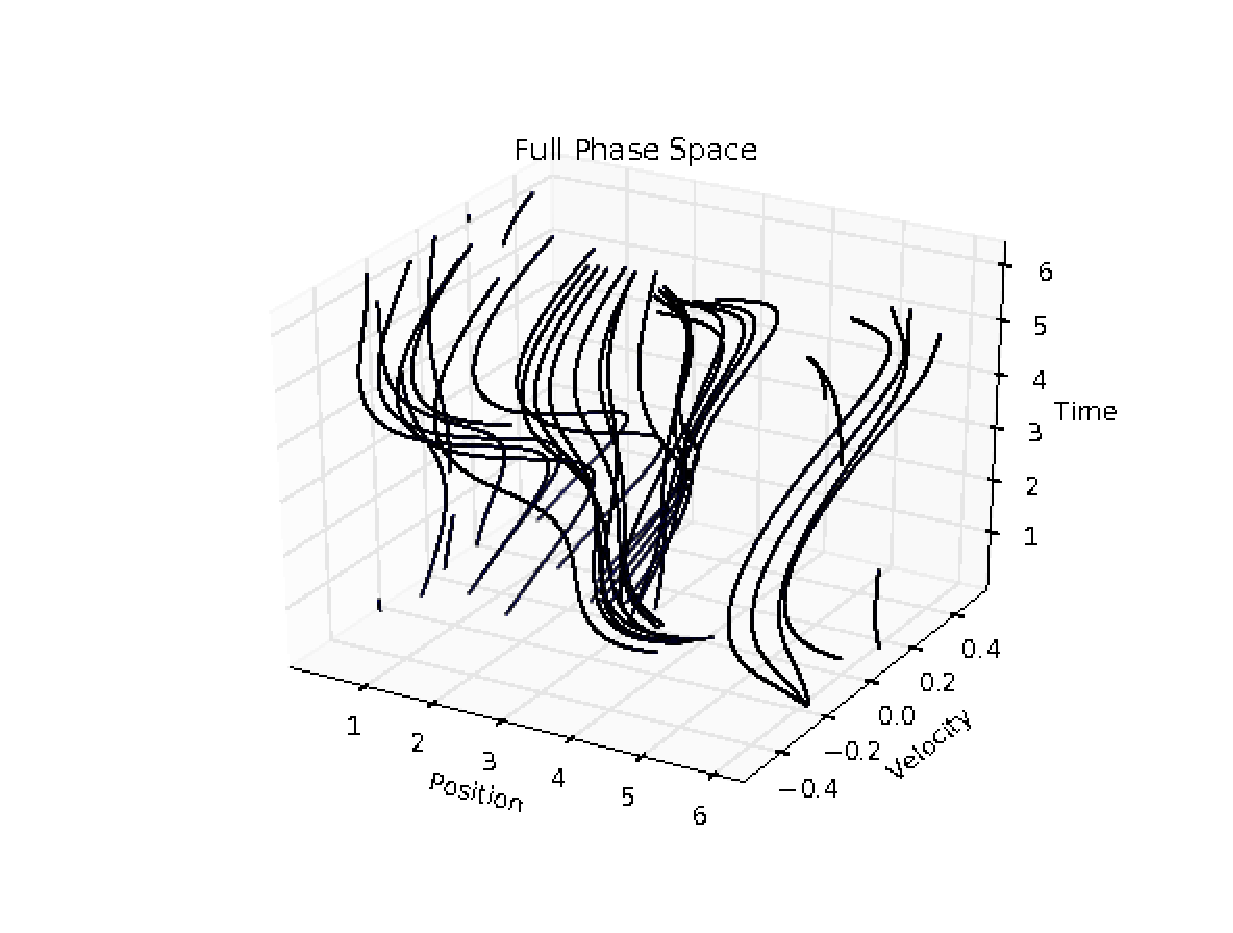
\includegraphics[width=3 in]{fullphasespaceEX}
    \caption{A particle trajectory periodic in time and space with $j=.272$}
    \label{3dimphase}
\end{figure}

A Poincar$\acute{e}$ section of the orbit shown in Fig. \ref{3dimphase} is obtained by plotting a cross section 
perpendicular to the time axis and parallel to the position and velocity axes. The orbit only
travels in one direction in time so we plot every intersection of the orbit shown in Fig.
\ref{3dimphase} with the plane chosen, which we arbitrarily put at $t=0$. The resulting
Poincar$\acute{e}$ section is shown in Fig. \ref{poincare1D}. The shape observed in Fig.
\ref{poincare1D}
is an example of a strange attractor. It is characteristic of chaotic systems with underlying order.
If one were to zoom in on a particular part of the strange attractor, it would exhibit the property
of self similarity, such that the curve repeats itself on ever smaller scales forming a fractal
geometry. Associated with any strange attractor is a domain of attraction, which are the set of
initial conditions that result in a particle approaching an orbit lying within the attractor. A nice
feature of this example is that experimentally this particular Poincar$\acute{e}$ section is easy to make by
simply taking a slice at one time throughout each period of the driving frequency, which is the same
thing as strobing the system at the driving frequency and then recording the particle velocity and
position at each strobe instant. We hope to verify some of our computations by doing just that. One
of the benefits of the 1D EC is the ability to view the full phase space graphically. When we look
at particle movement off the surface we end up with 5 first-order autonomous equations. We then have
to carefully choose how to project and slice the phase space to get useful information.


\begin{figure}[!t]
    \centering
    \includegraphics[width=3 in]{1DtimeSL}
    \caption{Poincar$\acute{e}$ section of trajectory shown in Fig. \ref{3dimphase}}
    \label{poincare1D}
\end{figure}

\subsection{Bifurcations}

One way to illustrate the system dynamics is with use of a bifurcation diagram, in which the value of
one variable (e.g., $x'$) on the Poincar$\acute{e}$ diagram is plotted as a function of a system
parameter (e.g., $j$). For small values of $j$ ($j<0.207$), the Poincar$\acute{e}$ diagram consists
of a single point, indicating a
periodic system with a single period, oscillating in phase with the driving frequency. As the
parameter $j$ is varied, the corresponding bifurcation plot appears as a single line as long as the
period stays in phase with the driving frequency. A period
doubling event occurs when the number of distinct frequencies in the oscillations increases by a
factor of two. A bifurcation plot for the 1D EC system is shown in Fig. 4 for $j$ in the interval
$0.200 < j < 0.221$. A period doubling event is found to occur at $j \approx 0.207$, beyond which the
Poincar$\acute{e}$
diagram for the system oscillates between two points, indicating two distinct system frequencies (or
period-2 orbit). A second period doubling occurs at $j=0.208$, beyond which the system is
characterized by four distinct frequencies (or period-4 orbit). In this second period doubling
event the periods appear to change in a discontinuous manner. The period-4 orbit appears to undergo
another period doubling event at $j = 0.210$, but on closer inspection we find that this is not the
case. Instead, the particle trajectory is found to remain a period-4 orbit, but as the value of $j$
changes the orbits periods are found to discontinuously jump between two sets of values, such that the
resulting shape on the bifurcation diagram appears as two dotted lines. Every blank spot in one of
these sets of lines coincides with a dot in the other set of lines. As $j$ is made higher still, the
system dynamics transitions back to a period-2 orbit. The sudden jumps in period values and number
of periods exhibited by this bifurcation diagram illustrates the very high level of sensitivity
exhibited by the electric curtain to changes in system properties in terms of the mode of particle
transport.

The bifurcation diagram is plotted in Fig. \ref{secondbif} for the medium-size interval $0.190<j<
0.275$ and in
Fig. \ref{thirdbif} for the large interval $0.190<j< 1.700$. In many systems that exhibit period
doubling behaviors,
onset of chaos occurs following a cascade of period doubling bifurcations that leads to an 
infinite period orbit. While numerous period doubling events are apparent in Figs.
\ref{firstbif}-\ref{thirdbif}, the onset of
chaos nevertheless seems to appear quite suddenly near $j=0.260$ (Fig. \ref{secondbif}). In Fig.
\ref{thirdbif}, it is shown
that following a relatively short interval of chaotic motion, the system again returns to a period-2
orbit, and than at much higher values of $j$ (near $j= 1.495$) the motion again becomes chaotic. 


\begin{figure}
    \centering
    \includegraphics[width=3 in]{firstbif}
    \caption{Bifurcation diagram for $0.200<j<0.221$}
    \label{firstbif}
\end{figure}

\begin{figure}[!t]
    \centering
    \includegraphics[width=3 in]{secondbif}
    \caption{Bifurcation diagram $0.190<j<0.275$}
    \label{secondbif}
\end{figure}

\begin{figure}[!t]
    \centering
    \includegraphics[width=3 in]{thirdbif}
    \caption{Bifurcation diagram $0.190<j<1.700$}
    \label{thirdbif}
\end{figure}


\section{Two Dimensional Electric Curtain}

The 1D EC model loses validity when particles start to hop off of the surface, which occurs for
approximately $j/g'>0.448$ for the surface at $y'=1$. For the 2D system we include
gravity and we set the ratio $j/g'$ to $3.06$ so we are in the regime of out of plane motion. The
particular parameters we use for the work shown here are $j=0.3$, $g'=0.1$, $\beta'=0.03$. The phase
space of the 2D system occupies a 5th order space, which makes analysis
considerably harder than for the 1D model. There should be some regime in which the particle leaves
the surface but is close enough that the 1D model approximates it. By looking for similarities in
Poincar$\acute{e}$ sections of the two models we hope to determine the full range of $j/g'$ above
$0.448$ for which the 1D model is appropriately valid. We are currently working on defining this
range in order to fully
exploit the simplicity of the 1D model. This information will be useful in future experimental comparisons.

Poincar$\acute{e}$ sections of the 2D EC
computations are obtained by plotting the particle positions at fixed time increments. Results are
shown in Figs \ref{2Dxslice} and \ref{2Dyslice}. The $x'$ velocity component is plotted against the
$x'$
position of the particle in Fig. \ref{2Dxslice}, and the $y'$ velocity component is plotted against
the $y'$ position of the particle in Fig. \ref{2Dyslice}. In order to deal with the surface
discontinuity that would appear in Fig. \ref{2Dyslice}, after bouncing from the
surface the particle motion is folded over the
surface position in constructing the Poincar$\acute{e}$ section. Hence, while a bounced particle is actually
located above the surface and moving upward, it is plotted in Fig. \ref{2Dyslice} as having
locations below the
dielectric surface with a downward velocity. The particles initially exhibit transient behavior, but
over long time settle into a regular pattern characteristic of an attractor. The transient behavior
produces scattered points on the Poincar$\acute{e}$ diagram, and the attractor yields points that form the
closed curves in Figs. \ref{2Dxslice} and \ref{2Dyslice}. The boundary of the attractor appears to
fold back on itself at
different intervals and to have a complex shape. 

\begin{figure}[!t]
    \centering
    \includegraphics[width=3 in]{2Dxslice}
    \caption{A Poincar$\acute{e}$ section parallel to the $x'$, $\dot{x}'$ phase plane and perpendicular to
        the time axis.}
    \label{2Dxslice}
\end{figure}

\begin{figure}[!t]
    \centering
    \includegraphics[width=3 in]{2Dyslice}
    \caption{A Poincar$\acute{e}$ section parallel to the $y'$, $\dot{y}'$ phase plane and perpendicular to
        the time axis.}
    \label{2Dyslice}
\end{figure}

   
    
\section{Conclusion}

A dynamical systems study of particle transport on an electric curtain has been initiated, and some
preliminary results are reported for both 1D and 2D particle transport. With use of bifurcation
diagrams, we have shown that the system undergoes a series of period doubling bifurcations, which
in some cases lead to intervals of chaotic dynamics and in other cases reverts back to a simple
finite period orbit. Poincar$\acute{e}$ sections are plotted which illustrate the presence of
strange attractors in
both 1D and 2D systems under chaotic transport conditions. We hope to continue our research of the
simple 2D model, as well as to explore more complex cases with particle-particle collisions and
multiple particles sizes, with the hope that by better understanding the dynamics of such systems we
will be better able to design electric curtain devices for optimal particle transport, mixing and
separation operations. 

\section*{Acknowledgment}
This work has been supported by NASA under cooperative agreement number NNX08AZ07A.
% \vfill\break


%As of right now we can only draw a
%comparison to the double tent map.
%TENT MAP FIGURE HERE.
%In the case of the doble tent map there is a discontinuity when the minimum between the two peaks
%and the second peak are draged across the y=x line. The number of intersections of the tent map with
%y=x determines the number of fixed points. When the relevent segemt of the map is aligned to y=x
%there are an infinite number of fixed points but as soon as the verticies pass this particular
%configuration the we jump back to a finite number of fixed points. In addition to the interesting
%rout to chaos we see a really nice strange atractor.












%TRAVE PLANE CHARGE
%(we should give that a name and symbol). The multi phase EC have some interesting
%dynamics but it is hard to look for interesting features in one dimension because there is an
%extremely robust attractor shown in figure \ref{travplaneattract}
%
%\begin{figure}[!t]
%    \centering
%    \includegraphics[width=2.5in]{travplanechargeattractor}
%    \caption{The robust attractor in the traveling plane charge approximation}
%    \label{travplaneattract}
%\end{figure}



% An example of a floating figure using the graphicx package.junru wu uvm
% Note that \label must occur AFTER (or within) \caption.
% For figures, \caption should occur after the \includegraphics.
% Note that IEEEtran v1.7 and later has special internal code that
% is designed to preserve the operation of \label within \caption
% even when the captionsoff option is in effect. However, because
% of issues like this, it may be the safest practice to put all your
% \label just after \caption rather than within \caption{}.
%
% Reminder: the "draftcls" or "draftclsnofoot", not "draft", class
% option should be used if it is desired that the figures are to be
% displayed while in draft mode.
%

%\begin{figure}[!t]
%\centering
%\includegraphics[width=2.5in]{myfigure}
% where an .eps filename suffix will be assumed under latex, 
% and a .pdf suffix will be assumed for pdflatex; or what has been declared
% via \DeclareGraphicsExtensions.
%\caption{Simulation Results}
%\label{fig_sim}
%\end{figure}

% Note that IEEE typically puts floats only at the top, even when this
% results in a large percentage of a column being occupied by floats.


% An example of a double column floating figure using two subfigures.
% (The subfig.sty package must be loaded for this to work.)
% The subfigure \label commands are set within each subfloat command, the
% \label for the overall figure must come after \caption.
% \hfil must be used as a separator to get equal spacing.
% The subfigure.sty package works much the same way, except \subfigure is
% used instead of \subfloat.
%
%\begin{figure*}[!t]
%\centerline{\subfloat[Case I]\includegraphics[width=2.5in]{subfigcase1}%
%\label{fig_first_case}}
%\hfil
%\subfloat[Case II]{\includegraphics[width=2.5in]{subfigcase2}%
%\label{fig_second_case}}}
%\caption{Simulation results}
%\label{fig_sim}
%\end{figure*}
%
% Note that often IEEE papers with subfigures do not employ subfigure
% captions (using the optional argument to \subfloat), but instead will
% reference/describe all of them (a), (b), etc., within the main caption.


% An example of a floating table. Note that, for IEEE style tables, the 
% \caption command should come BEFORE the table. Table text will default to
% \footnotesize as IEEE normally uses this smaller font for tables.
% The \label must come after \caption as always.
%
%\begin{table}[!t]
%% increase table row spacing, adjust to taste
%\renewcommand{\arraystretch}{1.3}
% if using array.sty, it might be a good idea to tweak the value of
% \extrarowheight as needed to properly center the text within the cells
%\caption{An Example of a Table}
%\label{table_example}
%\centering
%% Some packages, such as MDW tools, offer better commands for making tables
%% than the plain LaTeX2e tabular which is used here.
%\begin{tabular}{|c||c|}
%\hline
%One & Two\\
%\hline
%Three & Four\\
%\hline
%\end{tabular}
%\end{table}


% Note that IEEE does not put floats in the very first column - or typically
% anywhere on the first page for that matter. Also, in-text middle ("here")
% positioning is not used. Most IEEE journals/conferences use top floats
% exclusively. Note that, LaTeX2e, unlike IEEE journals/conferences, places
% footnotes above bottom floats. This can be corrected via the \fnbelowfloat
% command of the stfloats package.







% conference papers do not normally have an appendix


% use section* for acknowledgement
%\section*{Acknowledgment}







% trigger a \newpage just before the given reference
% number - used to balance the columns on the last page
% adjust value as needed - may need to be readjusted if
% the document is modified later
%\IEEEtriggeratref{8}
% The "triggered" command can be changed if desired:
%\IEEEtriggercmd{\enlargethispage{-5in}}

% references section

% can use a bibliography generated by BibTeX as a .bbl file
% BibTeX documentation can be easily obtained at:
% http://www.ctan.org/tex-archive/biblio/bibtex/contrib/doc/
% The IEEEtran BibTeX style support page is at:
% http://www.michaelshell.org/tex/ieeetran/bibtex/
%\bibliographystyle{IEEEtran}
% argument is your BibTeX string definitions and bibliography database(s)
%\bibliography{IEEEabrv,../bib/paper}
%
% <OR> manually copy in the resultant .bbl file
% set second argument of \begin to the number of references
% (used to reserve space for the reference number labels box)
%\begin{thebibliography}{1}

%\bibitem{IEEEhowto:kopka}
%H.~Kopka and P.~W. Daly, \emph{A Guide to \LaTeX}, 3rd~ed.\hskip 1em plus
%  0.5em minus 0.4em\relax Harlow, England: Addison-Wesley, 1999.

%\end{thebibliography}


\bibliographystyle{IEEEtran}
\bibliography{IEEEabrv,myrefs}




% that's all folks
\end{document}


